\chapter{Teil2}
\label{cha:Physikalische Grundlagen}



\begin{normalsize}


\section{Modell}
\label{sec:Modell}


\subsection{Stofftransport}

Die im untersuchten Enthalpieübertrager verwendete Membran besteht aus einer dichten Grundschicht und einer porösen Stützschicht. Der Stofftransport lässt sich analog zur Elektrotechnik als eine Kette von in Reihe geschalteten Prozessen darstellen. Eine Übersicht über die in Reihe geschalteten Prozesse gibt Abbildung\ref{fig:Transportprozesse}.
% Bild zu Membranprozessen einfügen

\begin{figure} [h]
	%\centering
	\caption{Transportprozesse}
	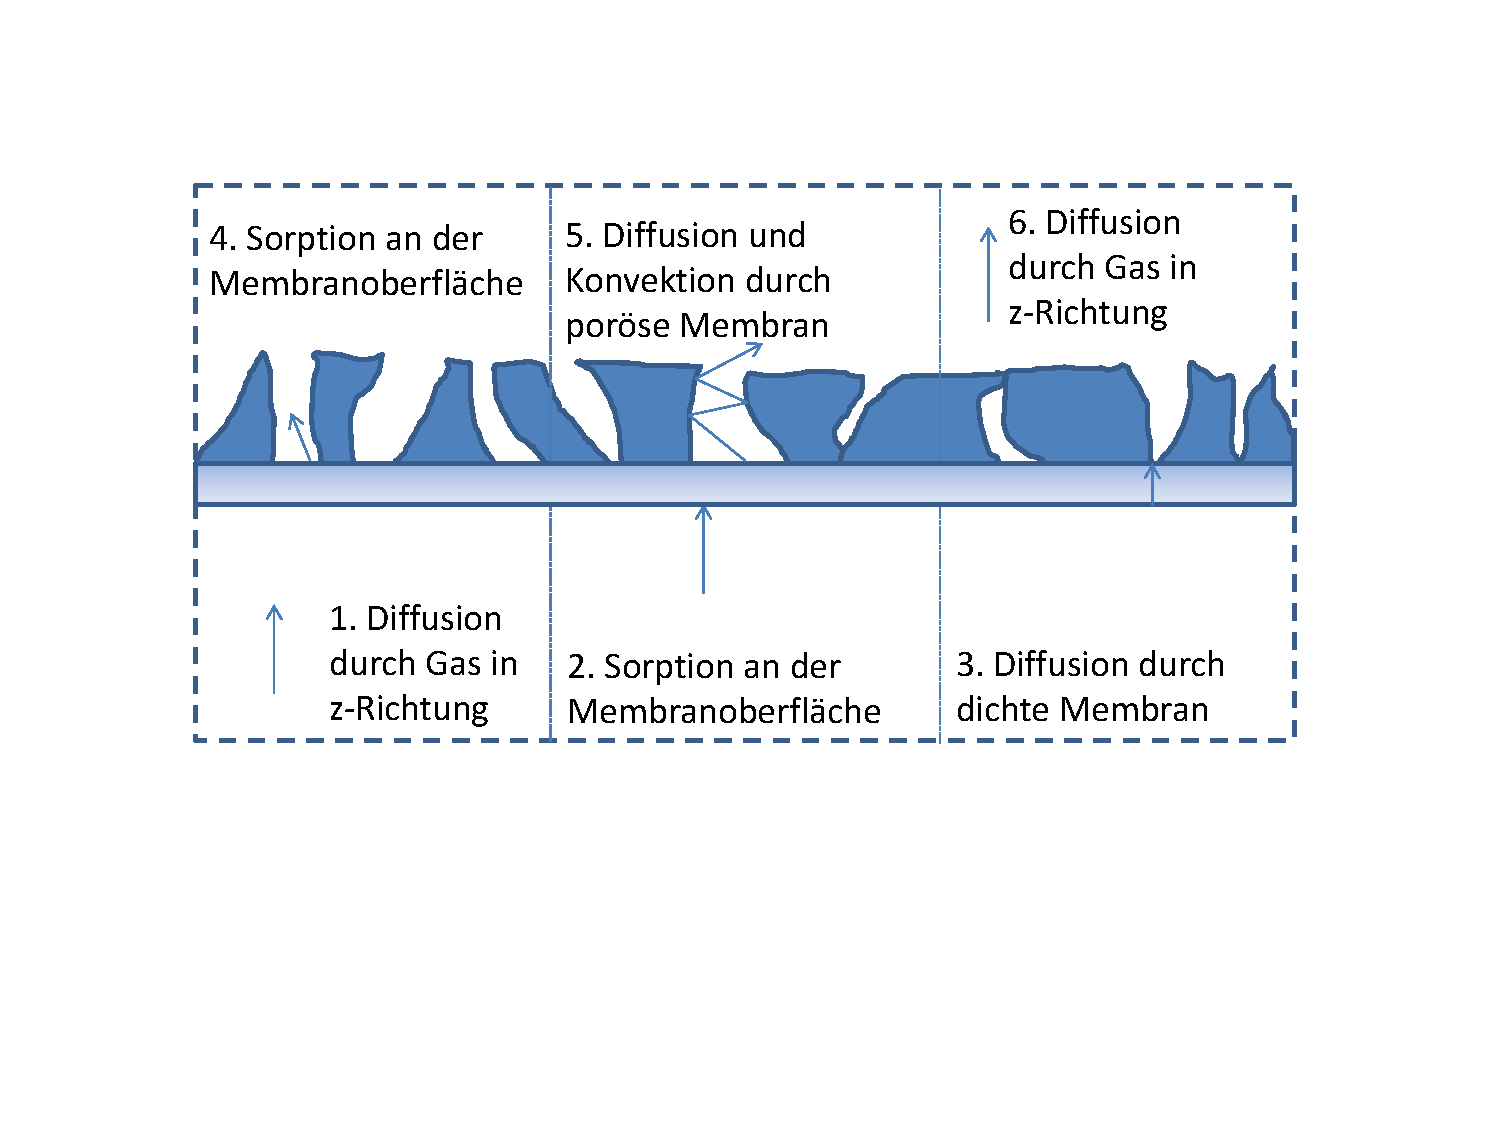
\includegraphics[width=0.98\textwidth]{pictures/Membran_Transportprozesse.pdf}
	
	\label{fig:Transportprozesse}
\end{figure}

Im ersten Schritt diffundiert der Wasserdampf durch den Luftstrom der Feedseite. Dies geschieht auf Grund eines Konzentrationsgradienten. Der Konzentrationsgradient entsteht durch das Ableiten des Wassermassenstroms durch die Membran. 

In einem zweiten Schritt absorbiert die Membranoberfläche den Wasserdampf. 

Im dritten Schritt folgt die Diffusion durch die dichte Grundschicht der Membran. 

Im vierten Schritt desorbiert das Wasser an der sweepseitigen Oberfläche der Membran in die Luft. 

In einem fünften Schritt wird der Wasserdampf durch die poröse Membran transportiert und verteilt sich in einem sechsten Schritt im Sweepstrom. Diese Diffusionsprozesse durch die Poren und den Luftstrom werden durch Konzentrationsgradienten verursacht.


Wie oben beschrieben führt die Betrachtung der 6 Prozessschritte als Reihenschaltung zu einer zutreffenden Beschreibung des Stofftransportes. Dies geschieht analog zur Elektrotechnik. Entsprechend ergibt sich der Gesamtwiderstand $W_{ges}$ der Membran 

\begin{equation}
 W_{ges} = W_{d} + W_{p}
\end{equation} 
 
aus einer Addition der Einzelwiderstände von dichter Membran $W_{d}$ und poröser Membran $W_{p}$.
 
Im Fall von parallel geschalteten Widerständen, zum Beispiel beim Auftreten von Poren in der dichten Membran, kann der Gesamtwiderstand analog zu 

\begin{equation}
\frac{1}{W_{ges}} = \frac{1}{W_{d}} + \frac{1}{W_{p}}
\end{equation}

gebildet werden. Beispiele hierfür sind das Auftreten von Poren in einer dichten Membran oder allgemein das parallele Stattfinden von konvektiven und diffusiven Stofftransportprozessen.


\subsubsection{Sorption an Membranoberfläche}
%Die Triebkraft des Sorptionsprozesses ist eine Differenz im chemischen Potential. Zur Beschreibung der Sorptionsprozesse werden meistens empirische und halbempirische Modelle genutzt. Das chemische Potential hängt im Fall der Sorption wesentlich von zwei Faktoren ab. Zum eine von der maximalen Wasserbeladung der Me
Die Triebkraft des Sorptionsprozesses ist eine Differenz im chemischen Potential. Meist werden hydrophile Membranenmaterialien für die dichte Membran eingesetzt. Daher entsteht an der Feed-Seite eine höherer Potentialdifferenz. Neben der Affinität des Membranmaterials ist die maximale Aufnahmekapazität der Membran ausschlaggebend für die Gleichgewichtskonzentration des Wassers in der Membranoberfläche. Dieses Lösungs-Gleichgewichtsmodell ist insbesondere von Lösungen anderer Aggregatzustände bekannt, z.B. von Salzlösungen oder Wasser-Luft-Lösungen. Die Beschreibung des Sorptionsprozesses mit physikalischen Modellen ist schwierig. Daher hat sich für die Beschreibung des Sorptionsprozesses ein halbempirisches Modell durchgesetzt, das sich in den meisten Veröffentlichungen wiederfindet, z.B. in \cite{J.L.Niu.2001} oder \cite{Dugaria.2015}. Demnach stellt sich in der Membranoberfläche eine Feuchtebeladung $\Theta$ von 

\begin{equation}
\Theta = \dfrac{\omega_{max}}{1-c+\frac{c}{\Phi}}
\end{equation}

ein. Wobei $\omega_{max}$ die maximal mögliche Feuchte im Membranmaterial angibt, $c$ eine Materialkonstante darstellt, die den Einfluss der Wasseraffinität der Membran wiederspiegelt, und $\Phi$ die Luftfeuchte im Luftstrom ist. 



\subsubsection{Diffusion durch dichte Membran}

Die Diffusion durch die dichte Membran ist im vorliegenden Fall der einflussreichste Prozessschritt auf die Transportgeschwindigkeit. Bei diesem Schritt ist der Widerstand am größten. Die Triebkraft ist hier - wie für alle Diffusionsprozesse - das chemische Potential. 
% ^ist das wirklich so?
%(Da die Wechselwirkungen mit der Temperatur gering sind und die es nicht zu relevanten chemischen Reaktionen kommt, kann der Partialdruck als Triebkraft angenommen werden. Im Fall von gleichem Druck auf beiden Seiten der Membran vereinfacht sich das System noch weiter und die Konzentration der Permeats in der Membranoberfläche kann als einzige relevante Triebkraft angesehen werden. 
%Daher resultiert der Permeatstrom J_{i} durch die Membran aus der Gleichung:
%\begin{equation}
%J_{i} = R*T*L_{i}/C_{i}*dC_{i}/dx
%\end{equation}

%in Abhängigkeit von der Gaskonstanten R, der Temperatur T und der Konzentration des Permeates i C_{i} und dessen örtlichen Gradienten dC_{i}/dx)

Unter der Annahme einer homogenen dichten Membran und konstanter thermodynamischer Randbedingungen (Druck und Temperatur) in der Membran ergibt sich eine lineare Konzentrationsverteilung über die Z-Achse der Membran. In der Literatur wird der Zusammenhang für den örtlichen Gradienten des chemischen Potentials und der übertragenen Stoffmenge ebenfalls als linear angenommen.(s.\cite{Koester.2015} 
%Literatur einfügen
%Da von konstanten thermodynamischen Eigenschaften in der Membran ausgegangen wird, ist es für die Modellierung egal ob der Massenstrom oder der Stoffmengenstrom betrachtet wird. 
Entsprechend ist für den Stoffmengentransport aus physikalischen Membranmodellen die Gleichung 

\begin{equation}
 \dot{n}^{\prime\prime} = - c_{wM} * b_{wM} * \frac{d\mu_{wM}}{dz}
\end{equation}

bekannt, wobei $\dot{n}^{\prime\prime}$ der Stoffmengenstrom des Wassers über die Membran ist und $b_{wM}$ die Beweglichkeit der diffundierenden Moleküle angibt. \cite{T.Melin.2007}
% hier: Nernst-Einstein, evtl noch auf Fick eingehen
Für den Diffusionsmassenstrom $J_{w}$ ergibt sich ein proportionaler Zusammenhang zum Gradienten des chemischen Potentials $\mu$

\begin{equation}
J_{w} = -L_{w}*\frac{d\mu_{w}}{dx}
\end{equation},

wobei $L_{w}$ der Proportionalitätsfaktor ist.

Das chemische Potential eines Stoffes $i$ ist definiert als Summe aus einem druckabhängigen Potentialterm, einem Standardpotentialterm und einem konzentrationsabhängigen Potentialterm zu

\begin{equation}
\mu_{i}(T,p,c_{i}) = \mu_{i}^\circ (T,p^\circ) + R*T*ln(a_{i}(T,p^\circ,c_{i})) + v_{i}*(p-p^\circ)
\end{equation},


wobei $P^\circ$ der Standarddruck ist, $R$ die ideale Gaskonstante \footnote{Gaskonstante = 8.314 J/mol/K}, $a_{i}$ die Aktivität des Stoffes $i$ und $v_{i}$ das Molvolumen des Stoffes $i$.


Der Druckterm
% würden sonst Einfluss auf die Durchmischung nehmen, da es die Geschw. d. Moleküle wiederspiegelt

\begin{equation}
v_{i}*(p-p^\circ)= 0
\end{equation}

entfällt unter der Voraussetzung einer idealen Gasmischung.

Der Standardpotentialterm $\mu_{i}^\circ(T,p^\circ)$ entfällt unter der Annahme von Isothermie entlang der z-Achse über die Membran. Da die dichte Membran sehr dünn ist, ist diese Annahme gerechtfertigt.
% Quellenangabe, evtl. Quelle 8 aber auch die Treffen eigentlich diese Annahme auch wenn sie Stoff und Wärmtransport koppeln wollen
% geringes delta T über mü, p0 auf beiden seiten gleich

Der konzentrationsabhängige Potentialterm hängt im Wesentlichen von der Aktivität der diffundierenden Komponente ab. Die Aktivität ist für Lösungen als
\begin{equation}
a_{i} = \gamma_{i}  * c_{i}
\end{equation}

definiert, wobei $\gamma_{i}$ der Aktivitätskoeffizient der Komponente $i$ ist. Der Aktivitätskoeffizient gibt das Verhältnis aus aktivem und realem Stoffmengenanteil an. Er nähert sich für kleine Konzentrationen dem Wert Eins. Da eine dichte Membran betrachtet wird, ist die Annahme sinnvoll.
Die oben beschriebenen Annahmen wurden auch von Zhang und Niu getroffen und mit experimentellen Ergebnissen validiert \cite{Zhang.2002b}. 

Aus den Annahmen folgt, dass der konzentrationsabhängige Potentialterm sich zu 

\begin{equation}
RT*ln(a_{i}(T,p^\circ,c_{i})) = RT*ln(c_{i})
\end{equation}

vereinfacht.

Unter den getroffenen Annahmen ergibt sich für den Stoffmengentransport von Wasser durch die Membran die Gleichung
%Detaillierter?
\begin{equation}
J_{w} = \frac{-L_{w}*RT}{c_{w}} * \frac{d c_{w}}{dx}
\end{equation}.

Daher lässt sich unter der Voraussetzung einer linearen Verteilung von $c_{w}$ über die z-Richtung der Membran ein linearer Zusammenhang des Stoffmengentransports von der Konzentrationsdifferenz mit einem Diffusionskoeffizienten $D_{w}$ beschreiben. So folgt die Gleichung:
\begin{equation}
J_{w} = D_{w} * \dfrac{c_{wfm}-c_{wsm}}{\delta}
\end{equation},

wobei $c_{wfm}$ und $c_{wsm}$ die Stoffmengenkonzentrationen in der feedseitigen beziehungsweise in der sweepseitigen Membranoberfläche darstellen.


\subsubsection{Diffusion durch poröse Membran}

Der Stofftransport durch die poröse Membran setzt sich aus einem Diffusionsprozess und einem Konvektionsprozess zusammen. Eine Konvektion in x- oder y-Richtung findet auf Grund der Porenausrichtung nicht statt. Die Konvektion in z-Richtung entsteht durch den Permeatstrom. Die Diffusion ergibt sich auf Grund des Konzentrationsgradienten. 

\subsubsection{Stofftransport im Luftstrom}

Bei der Beschreibung des Transports der Wassermoleküle durch die Gasphase führt die Annahme einer laminaren Luftströmung in x-Richtung zu einer deutlichen Vereinfachung des Modells. Im Fall laminarer Strömung kommt es nicht zum konvektiven Stoffaustausch in z-Richtung. Der Transport der Wassermoleküle in z-Richtung lässt sich unter dieser Annahme mit Hilfe von Diffusionsmodellen beschreiben.
Die Betrachtung turbulenter Stofftransportprozesse ist in der Regel mit aufwendigen Strömungssimulationen verbunden. Eine Beschränkung auf laminare Effekte kann somit den Rechenaufwand bei Simulationen erheblich reduzieren. 

Da die Turbulenz stark von der Geometrie  des Strömungskanals und der Strömungsgeschwindigkeit abhängt, ist diese Annahme nicht uneingeschränkt gültig. Insbesondere Spacermaterialien werden bewusst dazu eingesetzt, die Turbulenz in den Strömungskanälen zu erhöhen.
Eine erhöhte Turbulenz führt zu einer Abnahme der Konzentrationsüberhöhung an den Membranoberflächen und wirkt sich positiv auf die Sorptionsgeschwindigkeit an der Membranoberfläche aus.  

%Bild zur Konzentrationspolarisation einfügen
  
Konzentrationsüberhöhungen entstehen durch einen konvektiven Fluss. Der Permeatfluss durch die Membran zieht auf Grund der Kontinuitätsgleichungen einen konvektiven Massenstrom in z-Richtung nach sich. Da die Membran selektiv ist, diffundieren nur einige Stoffe, in diesem Fall die Wassermoleküle durch die Membran. Entsprechend nimmt die Konzentration der anderen Stoffe an der Membranoberfläche zu. Der Konzentrationsgradient des Wassers über die Membran ist daher geringer und somit auch die Triebkraft des Stofftransportes. Die Auswirkungen der Konzentrationspolarisation sind aber im hier betrachteten Fall gering, da der Permeatstrom im Vergleich zum Gesamtmassenstrom gering ist. 
%^noch mal prüfen und permeatstrom evtl. durch Diffusionsstrom o.Ä. ersetzen


\subsection{Zusammenfassend}


                                                                                               


\end{normalsize}


























 